\section{Preventivo}
\label{preventivo}
Per ogni periodo individuato nella sezione \S\ref{pianificazione} relativa alla pianificazione, si espone un prospetto orario dove sono raccolte le ore che ciascun membro deve svolgere per ruolo.\\Viene successivamente mostrato un prospetto economico che riassume i costi sostenuti per ciascun ruolo.\\
Per agevolare la lettura delle tabelle, se un membro del gruppo non ha ricoperto un certo ruolo verrà inserito il simbolo \textbf{-} per indicarne l'assenza.\\Si è poi pensato di utilizzare le seguenti sigle per identificare i ruoli:
\begin{itemize}
\item \textbf{Re:} \textit{\Responsabile};
\item \textbf{Am:} \textit{\Amministratore};
\item \textbf{An:} \textit{Analista};
\item \textbf{Pt:} \textit{Progettista};
\item \textbf{Pr:} \textit{Programmatore};
\item \textbf{Ve:} \textit{Verificatore}.
\end{itemize}
\newpage

\subsection{Periodo di Analisi}
\subsubsection{Prospetto orario}
In questo periodo, ogni componente del gruppo rivestirà i seguenti ruoli:
\begin{table}[H]
	\begin{center}
		\begin{tabular}{ |c c c c c c c c|}
		\rowcolor{darkblue} 
		\textcolor{white}{\textbf{Nominativo}} & \textcolor{white}{\textbf{Re}} & \textcolor{white}{\textbf{Am}} & \textcolor{white}{\textbf{An}} & \textcolor{white}{\textbf{Pt}} & \textcolor{white}{\textbf{Pr}} & \textcolor{white}{\textbf{Ve}} & \textcolor{white}{\textbf{Ore Complessive}} \\ \hline
		\BL 	& - 	& 6 	& 16 	& - 	& - 	& 8 	& 30 \\ \hline
		\FF 	& - 	& 5 	& 15 	& - 	& - 	& 10 	& 30 \\ \hline
		\MM		& 15	& - 	& 10 	& - 	& - 	& 5 	& 30 \\ \hline
		\PC		& 5 	& 4 	& 10 	& - 	& - 	& 11	& 30 \\ \hline
		\TG 	& - 	& 15	& 10 	& - 	& - 	& 5 	& 30 \\ \hline
		\TL 	& 4 	& 5 	& 16 	& - 	& - 	& 5 	& 30 \\ \hline
		\VD 	& - 	& -  	& 12 	& - 	& - 	& 18 	& 30 \\ \hline
		\textbf{Ore totali} & \textbf{24} & \textbf{35} & \textbf{89} & \textbf{-} & \textbf{-} & \textbf{62} & \textbf{210} \\ \hline
		\end{tabular}
	\caption{Distribuzione delle ore nel periodo di Analisi}
	\end{center}
\end{table}
I dati ottenuti vengono riassunti nel seguente istogramma:
\begin{figure}[H]
    \centering
    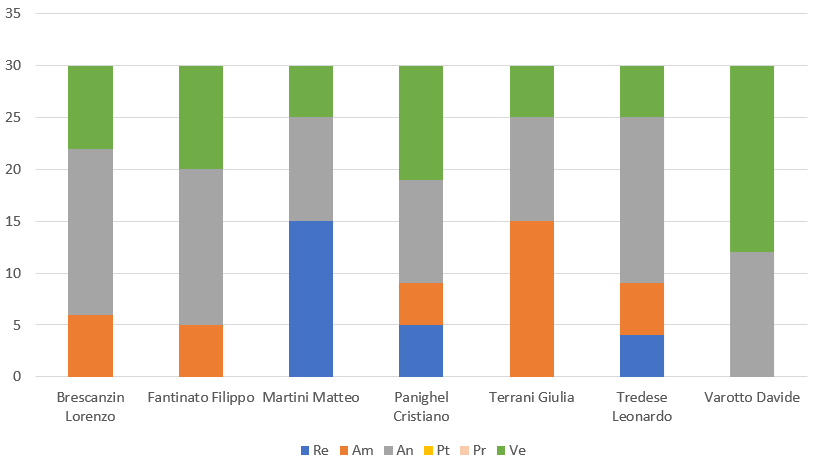
\includegraphics[scale = 0.70]{Immagini/AnalisiIsto.png}
    \caption{Istogramma della ripartizione delle ore per ruolo in Analisi}
    \label{fig:istogramma ripartizione ore, periodo di Analisi}
\end{figure}
\newpage
\subsubsection{Prospetto economico}
Il costo per ogni ruolo è il seguente:
\begin{table}[H]
	\begin{center}
		\begin{tabular}{ |c c c| }
		\rowcolor{darkblue} 
		\textcolor{white}{\textbf{Ruolo}} & \textcolor{white}{\textbf{Ore}} & \textcolor{white}{\textbf{Costo}} \\ \hline
		\textit{\Responsabile} 		& 24 	& 720€ \\ \hline
		\textit{\Amministratore} 	& 35 	& 700€ \\ \hline
		\textit{Analista} 			& 89 	& 2225€ \\ \hline
		\textit{Progettista} 		& - 	& - \\ \hline
		\textit{Programmatore}  	& - 	& - \\ \hline
		\textit{Verificatore} 		& 62 	& 930€ \\ \hline
		\textbf{Totale} 			& \textbf{210} & \textbf{4575€} \\ \hline
		\end{tabular}
	\caption{ Prospetto dei costi per ruoli nel periodo di Analisi}
	\end{center}
\end{table}
Il seguente grafico a torta riassume i dati ottenuti:
\begin{figure}[H]
    \centering
    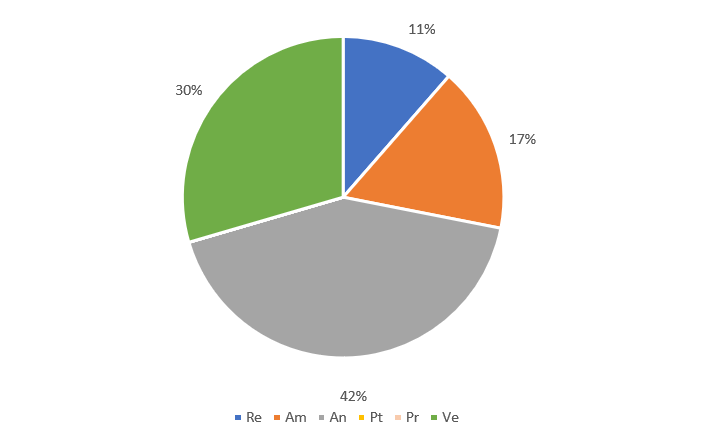
\includegraphics[scale = 0.75]{Immagini/AnalisiTorta.png}
    \caption{Areogramma ripartizione ore, periodo di Analisi}
    \label{fig:Areogramma ripartizione ore, periodo di Analisi}
\end{figure}
\newpage

\subsection{Periodo di Consolidamento dei Requisiti}
\subsubsection{Prospetto orario}
Durante il periodo di Consolidamento dei Requisiti viene effettuata la seguente distribuzione oraria:
\begin{table}[H]
	\begin{center}
		\begin{tabular}{ |c c c c c c c c| }
		\rowcolor{darkblue} 
		\textcolor{white}{\textbf{Nominativo}} & \textcolor{white}{\textbf{Re}} & \textcolor{white}{\textbf{Am}} & \textcolor{white}{\textbf{An}} & \textcolor{white}{\textbf{Pt}} & \textcolor{white}{\textbf{Pr}} & \textcolor{white}{\textbf{Ve}} & \textcolor{white}{\textbf{Ore Complessive}} \\ \hline
		\BL 	& - 	& 3  	& - 	& 3 	& - 	& - 	& 6 \\ \hline
		\FF 	& - 	& 3  	& 3 	& - 	& - 	& -  	& 6 \\ \hline
		\MM 	& -  	& -  	& 2 	& - 	& - 	& 4  	& 6 \\ \hline
		\PC 	& - 	& -  	& 4 	& 2 	& - 	& - 	& 6 \\ \hline
		\TG 	& 2  	& - 	& 4 	& - 	& - 	& - 	& 6 \\ \hline
		\TL 	& 3  	& - 	& - 	& - 	& - 	& 3 	& 6 \\ \hline
		\VD 	& -  	& -  	& 4 	& 2 	& - 	& -  	& 6 \\ \hline
		\textbf{Ore totali} & \textbf{5} & \textbf{6} & \textbf{17} & \textbf{7} & \textbf{-} & \textbf{7} & \textbf{42} \\ \hline
		\end{tabular}
	\caption{Distribuzione delle ore nel periodo di Consolidamento dei Requisiti}
	\end{center}
\end{table}
I dati ottenuti vengono riassunti nel seguente istogramma:
\begin{figure}[H]
    \centering
    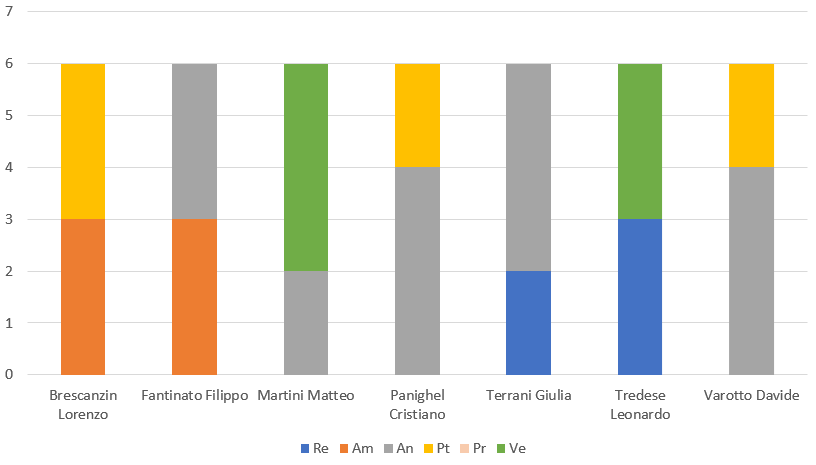
\includegraphics[scale = 0.70]{Immagini/ConsolidamentoIsto.png}
    \caption{Istogramma della ripartizione delle ore per ruolo in Consolidamento dei Requisiti}
    \label{fig:istogramma ripartizione ore, periodo di Consolidamento dei Requisiti}
\end{figure}
\newpage
\subsubsection{Prospetto economico}
Il costo per ogni ruolo è il seguente:
\begin{table}[H]
	\begin{center}
		\begin{tabular}{ |c c c|}
		\rowcolor{darkblue} 
		\textcolor{white}{\textbf{Ruolo}} & \textcolor{white}{\textbf{Ore}} & \textcolor{white}{\textbf{Costo}} \\ \hline
		\textit{\Responsabile} 		& 5 	& 150€ \\ \hline
		\textit{\Amministratore} 	& 6 	& 120€ \\ \hline
		\textit{Analista} 			& 17 	& 425€ \\ \hline
		\textit{Progettista} 		& 7 	& 154€ \\ \hline
		\textit{Programmatore}  	& - 	& - \\ \hline
		\textit{Verificatore} 		& 7 	& 105€ \\ \hline
		\textbf{Totale} 			& \textbf{42} & \textbf{954€} \\ \hline
		\end{tabular}
	\caption{ Prospetto dei costi per ruoli nel periodo di Consolidamento dei Requisiti}
	\end{center}
\end{table}
Il seguente grafico a torta riassume i dati ottenuti:
\begin{figure}[H]
    \centering
    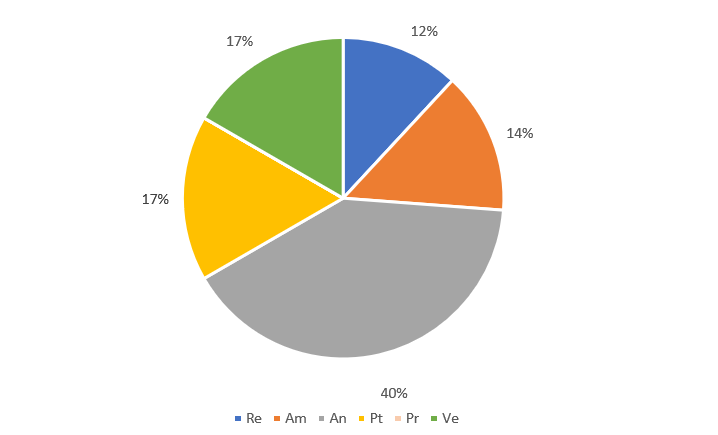
\includegraphics[scale = 0.75]{Immagini/ConsolidamentoTorta.png}
    \caption{Areogramma della ripartizione di ore per ruolo in Consolidamento dei Requisiti}
    \label{fig:Areogramma ripartizione ore, periodo di Consolidamento dei Requisiti}
\end{figure}
\newpage

\subsection{Periodo di Progettazione Architetturale}
\subsubsection{Prospetto orario}
In questo periodo la distribuzione oraria è la seguente:
\begin{table}[H]
	\begin{center}
		\begin{tabular}{ |c c c c c c c c| }
		\rowcolor{darkblue} 
		\textcolor{white}{\textbf{Nominativo}} & \textcolor{white}{\textbf{Re}} & \textcolor{white}{\textbf{Am}} & \textcolor{white}{\textbf{An}} & \textcolor{white}{\textbf{Pt}} & \textcolor{white}{\textbf{Pr}} & \textcolor{white}{\textbf{Ve}} & \textcolor{white}{\textbf{Ore Complessive}} \\ \hline
		\BL 	& -  	& -  	& 8 	& 12 	& 3 	& 7 	& 30 \\ \hline
		\FF 	& 3  	& -  	& - 	& 16 	& 5 	& 6  	& 30 \\ \hline
		\MM 	& -  	& 3  	& 10 	& 8 	& 5 	& 4  	& 30 \\ \hline
		\PC 	& - 	& -  	& 10 	& - 	& 4 	& 16 	& 30 \\ \hline
		\TG 	& -  	& 3 	& 10 	& 13 	& - 	& 4 	& 30 \\ \hline
		\TL 	& 5  	& 6 	& - 	& - 	& 4 	& 15 	& 30 \\ \hline
		\VD 	& 10  	& 8  	& - 	& 12 	& - 	& -  	& 30 \\ \hline
		\textbf{Ore totali} & \textbf{18} & \textbf{20} & \textbf{38} & \textbf{61} & \textbf{21} & \textbf{52} & \textbf{210} \\ \hline
		\end{tabular}
	\caption{Distribuzione delle ore nel periodo di Progettazione Architetturale}
	\end{center}
\end{table}
I dati ottenuti vengono riassunti nel seguente istogramma:
\begin{figure}[H]
    \centering
    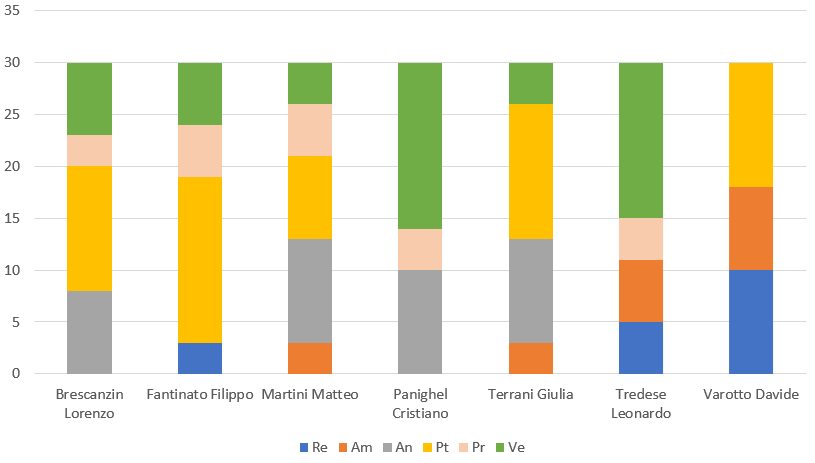
\includegraphics[scale = 0.70]{Immagini/ArchitetturaIsto.png}
    \caption{Istogramma della ripartizione delle ore per ruolo in Progettazione Architetturale}
    \label{fig:istogramma ripartizione ore, periodo di Progettazione Architetturale}
\end{figure}
\newpage
\subsubsection{Prospetto economico}
Il costo per ogni ruolo è il seguente:
\begin{table}[H]
	\begin{center}
		\begin{tabular}{ |c c c| }
		\rowcolor{darkblue} 
		\textcolor{white}{\textbf{Ruolo}} & \textcolor{white}{\textbf{Ore}} & \textcolor{white}{\textbf{Costo}} \\ \hline
		\textit{\Responsabile} 		& 18 & 540€ \\ \hline
		\textit{\Amministratore} 	& 20 & 400€ \\ \hline
		\textit{Analista} 			& 38 & 950€ \\ \hline
		\textit{Progettista} 		& 61 & 1342€\\ \hline
		\textit{Programmatore}  	& 21 & 315€ \\ \hline
		\textit{Verificatore} 		& 52 & 780€ \\ \hline
		\textbf{Totale} & \textbf{210} & \textbf{4327€} \\ \hline
		\end{tabular}
	\caption{ Prospetto dei costi per ruoli nel periodo di Progettazione Architetturale}
	\end{center}
\end{table}
Il seguente grafico a torta riassume i dati ottenuti:
\begin{figure}[H]
    \centering
    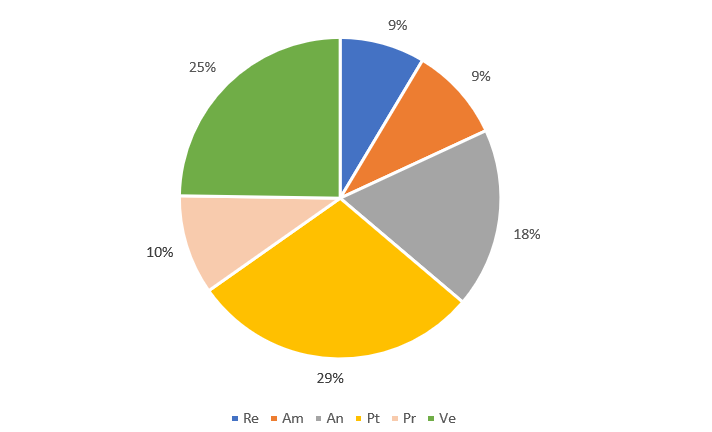
\includegraphics[scale = 0.75]{Immagini/ArchitetturaTorta.png}
    \caption{Areogramma della ripartizione di ore per ruolo in Progettazione Architetturale}
    \label{fig:Areogramma ripartizione ore, periodo di Progettazione Architetturale}
\end{figure}
\newpage

\subsection{Periodo di Progettazione di Dettaglio e Codifica}
\subsubsection{Prospetto orario}
In questo periodo la distribuzione oraria è la seguente:
\begin{table}[H]
	\begin{center}
		\begin{tabular}{ |c c c c c c c c| }
		\rowcolor{darkblue} 
		\textcolor{white}{\textbf{Nominativo}} & \textcolor{white}{\textbf{Re}} & \textcolor{white}{\textbf{Am}} & \textcolor{white}{\textbf{An}} & \textcolor{white}{\textbf{Pt}} & \textcolor{white}{\textbf{Pr}} & \textcolor{white}{\textbf{Ve}} & \textcolor{white}{\textbf{Ore Complessive}} \\ \hline
		\BL 	& 4  	& -  	& - 	& 15 	& 21 	& 10 	& 50 \\ \hline
		\FF 	& -  	& -  	& - 	& 30 	& 20 	& -  	& 50 \\ \hline
		\MM 	& -  	& 8  	& - 	& 15 	& 15 	& 12 	& 50 \\ \hline
		\PC 	& 5 	& 4  	& - 	& 11 	& 18 	& 12 	& 50 \\ \hline
		\TG 	& 5  	& 2		& - 	& 6 	& 20 	& 17 	& 50 \\ \hline
		\TL 	& -  	& - 	& - 	& 15 	& 20 	& 15 	& 50 \\ \hline
		\VD 	& 4  	& 4  	& - 	& 12 	& 20 	& 10 	& 50 \\ \hline
		\textbf{Ore totali} & \textbf{18} & \textbf{18} & \textbf{-} & \textbf{104} & \textbf{134} & \textbf{76} & \textbf{350} \\ \hline
		\end{tabular}
	\caption{Distribuzione delle ore nel periodo di Progettazione di Dettaglio e Codifica}
	\end{center}
\end{table}
I dati ottenuti vengono riassunti nel seguente istogramma:
\begin{figure}[H]
    \centering
    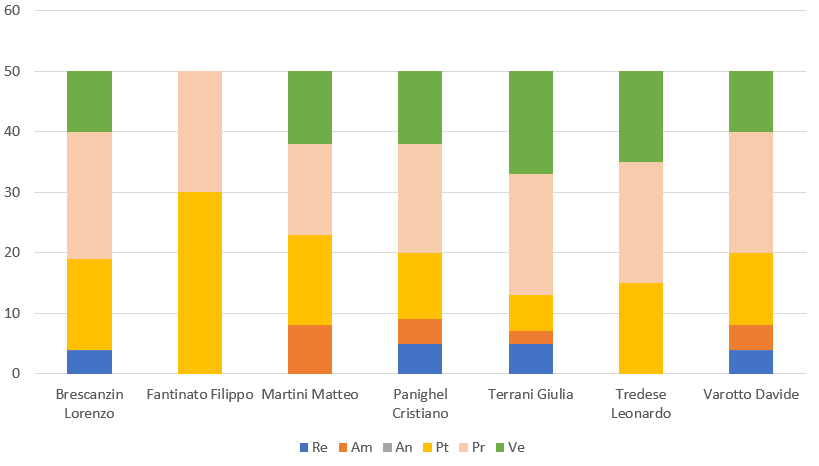
\includegraphics[scale = 0.70]{Immagini/DettaglioIsto.png}
    \caption{Istogramma della ripartizione delle ore per ruolo in Progettazione di Dettaglio e Codifica}
    \label{fig:istogramma ripartizione ore, periodo di Progettazione di Dettaglio e Codifica}
\end{figure}
\newpage
\subsubsection{Prospetto economico}
Il costo per ogni ruolo è il seguente:
\begin{table}[H]
	\begin{center}
		\begin{tabular}{ |c c c| }
		\rowcolor{darkblue} 
		\textcolor{white}{\textbf{Ruolo}} & \textcolor{white}{\textbf{Ore}} & \textcolor{white}{\textbf{Costo}} \\ \hline
		\textit{\Responsabile} 		& 18 	& 540€ \\ \hline
		\textit{\Amministratore} 	& 18 	& 360€ \\ \hline
		\textit{Analista} 			& - 	& - \\ \hline
		\textit{Progettista} 		& 104 	& 2288€ \\ \hline
		\textit{Programmatore}  	& 134 	& 2010€ \\ \hline
		\textit{Verificatore} 		& 76 	& 1140€ \\ \hline
		\textbf{Totale} & \textbf{350} & \textbf{6338€} \\ \hline
		\end{tabular}
	\caption{ Prospetto dei costi per ruoli nel periodo di Progettazione di Dettaglio e Codifica}
	\end{center}
\end{table}
Il seguente grafico a torta riassume i dati ottenuti:
\begin{figure}[H]
    \centering
    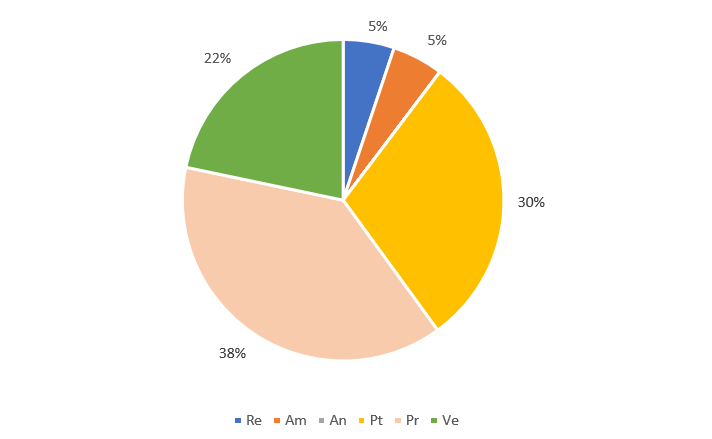
\includegraphics[scale = 0.75]{Immagini/DettaglioTorta.png}
    \caption{Areogramma della ripartizione di ore per ruolo in Progettazione di dettaglio e codifica}
    \label{fig:Areogramma ripartizione ore, periodo di Progettazione di Dettaglio e Codifica}
\end{figure}
\newpage

\subsection{Periodo di Validazione e Collaudo}
\subsubsection{Prospetto orario}
In questo periodo la distribuzione oraria è la seguente:
\begin{table}[H]
	\begin{center}
		\begin{tabular}{ |c c c c c c c c| }
		\rowcolor{darkblue} 
		\textcolor{white}{\textbf{Nominativo}} & \textcolor{white}{\textbf{Re}} & \textcolor{white}{\textbf{Am}} & \textcolor{white}{\textbf{An}} & \textcolor{white}{\textbf{Pt}} & \textcolor{white}{\textbf{Pr}} & \textcolor{white}{\textbf{Ve}} & \textcolor{white}{\textbf{Ore Complessive}} \\ \hline
		\BL 	& -  	& 5  	& - 	& 5 	& - 	& 10 	& 20 \\ \hline
		\FF 	& 4  	& 5  	& - 	& - 	& 5 	& 6  	& 20 \\ \hline
		\MM 	& 4 	& - 	& - 	& - 	& 6 	& 10  	& 20 \\ \hline
		\PC 	& 5 	& -  	& - 	& - 	& 7 	& 8 	& 20 \\ \hline
		\TG 	& -  	& 6 	& - 	& - 	& 8 	& 6 	& 20 \\ \hline
		\TL 	& -  	& - 	& - 	& 4 	& 6 	& 10 	& 20 \\ \hline
		\VD 	& 4  	& -  	& - 	& - 	& 4 	& 12  	& 20 \\ \hline
		\textbf{Ore totali} & \textbf{17} & \textbf{16} & \textbf{-} & \textbf{9} & \textbf{36} & \textbf{62} & \textbf{140} \\ \hline
		\end{tabular}
	\caption{Distribuzione delle ore nel periodo di Validazione e Collaudo}
	\end{center}
\end{table}
I dati ottenuti vengono riassunti nel seguente istogramma:
\begin{figure}[H]
    \centering
    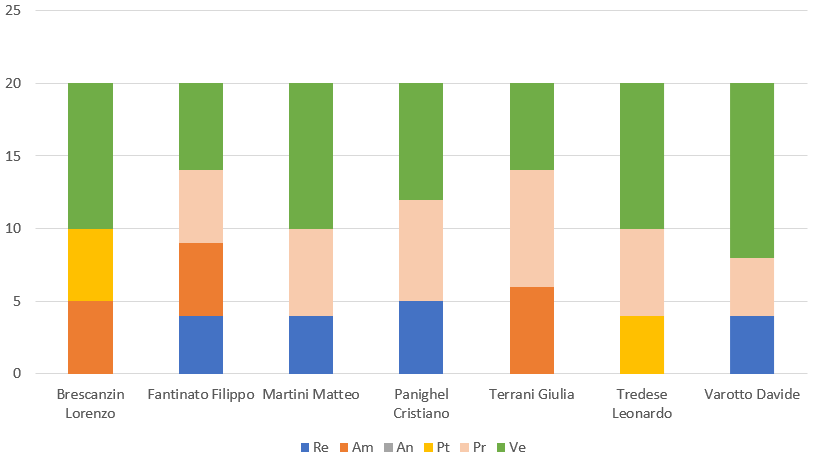
\includegraphics[scale = 0.70]{Immagini/ValidazioneIsto.png}
    \caption{Istogramma della ripartizione delle ore per ruolo in Validazione e collaudo}
    \label{fig:istogramma ripartizione ore, periodo di Validazione e Collaudo}
\end{figure}
\newpage
\subsubsection{Prospetto economico}
Il costo per ogni ruolo è il seguente:
\begin{table}[H]
	\begin{center}
		\begin{tabular}{ |c c c| }
		\rowcolor{darkblue} 
		\textcolor{white}{\textbf{Ruolo}} & \textcolor{white}{\textbf{Ore}} & \textcolor{white}{\textbf{Costo}} \\ \hline
		\textit{\Responsabile} 		& 17 	& 510€ \\ \hline
		\textit{\Amministratore} 	& 16 	& 320€ \\ \hline
		\textit{Analista} 			& - 	& - \\ \hline
		\textit{Progettista} 		& 9 	& 198€ \\ \hline
		\textit{Programmatore}  	& 36 	& 540€ \\ \hline
		\textit{Verificatore} 		& 62 	& 930€ \\ \hline
		\textbf{Totale} & \textbf{140} & \textbf{2498€} \\ \hline
		\end{tabular}
	\caption{ Prospetto dei costi per ruoli nel periodo di Validazione e Collaudo}
	\end{center}
\end{table}
Il seguente grafico a torta riassume i dati ottenuti:
\begin{figure}[H]
    \centering
    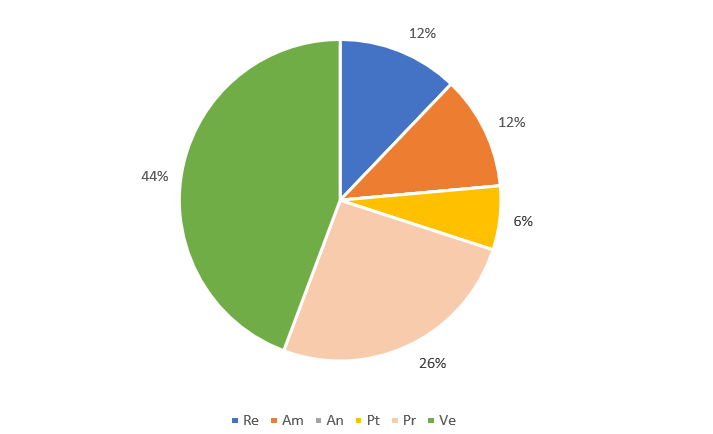
\includegraphics[scale = 0.75]{Immagini/ValidazioneTorta.png}
    \caption{Areogramma della ripartizione di ore per ruolo in Validazione e Collaudo}
    \label{fig:Areogramma ripartizione ore, periodo di Validazione e Collaudo}
\end{figure}
\newpage

\subsection{Riepilogo}
\subsubsection{Ore totali}
\paragraph{Suddivisione del lavoro}
Nella seguente tabella vengono riportate il totale delle ore del progetto, sono presenti sia le ore di investimento, sia le ore rendicontate a carico del committente.
\begin{table}[H]
	\begin{center}
		\begin{tabular}{ |c c c c c c c c| }
		\rowcolor{darkblue} 
		\textcolor{white}{\textbf{Nominativo}} & \textcolor{white}{\textbf{Re}} & \textcolor{white}{\textbf{Am}} & \textcolor{white}{\textbf{An}} & \textcolor{white}{\textbf{Pt}} & \textcolor{white}{\textbf{Pr}} & \textcolor{white}{\textbf{Ve}} & \textcolor{white}{\textbf{Ore Complessive}} \\ \hline
		\BL 	& 4  	& 14  	& 24 	& 35 	& 24 	& 35 	& 136 \\ \hline
		\FF 	& 7 	& 13 	& 18 	& 46 	& 30 	& 22 	& 136 \\ \hline
		\MM 	& 19  	& 11  	& 22 	& 23 	& 26 	& 35  	& 136 \\ \hline
		\PC 	& 15 	& 8  	& 24 	& 13 	& 29	& 47 	& 136 \\ \hline
		\TG 	& 7  	& 26 	& 24 	& 19 	& 28 	& 32 	& 136 \\ \hline
		\TL 	& 12  	& 11 	& 16 	& 19 	& 30 	& 48 	& 136 \\ \hline
		\VD 	& 18  	& 12  	& 16 	& 26 	& 24 	& 40 	& 136 \\ \hline
		\textbf{Ore totali} & \textbf{82} & \textbf{95} & \textbf{144} & \textbf{181} & \textbf{191} & \textbf{259} & \textbf{952} \\ \hline
		\end{tabular}
	\caption{Distribuzione delle ore totali di investimento e rendicontate}
	\end{center}
\end{table}
I dati ottenuti vengono riassunti nel seguente istogramma:
\begin{figure}[H]
    \centering
    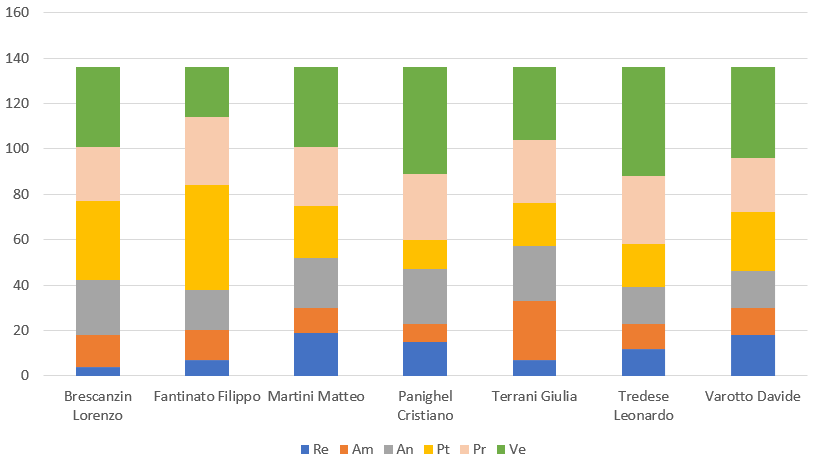
\includegraphics[scale = 0.70]{Immagini/TotaleIsto.png}
    \caption{Istogramma della ripartizione delle ore totali di investimento e rendicontate}
    \label{fig:Istogramma ripartizione ore totali di investimento e rendicontate }
\end{figure}
\newpage
\paragraph{Prospetto economico}
Il costo per ogni ruolo è il seguente:
\begin{table}[H]
	\begin{center}
		\begin{tabular}{ |c c c| }
		\rowcolor{darkblue} 
		\textcolor{white}{\textbf{Ruolo}} & \textcolor{white}{\textbf{Ore}} & \textcolor{white}{\textbf{Costo}} \\ \hline
		\textit{\Responsabile} 		& 82 	& 2460€ \\ \hline
		\textit{\Amministratore} 	& 95 	& 1900€ \\ \hline
		\textit{Analista} 			& 144 	& 3600€ \\ \hline
		\textit{Progettista} 		& 181 	& 3982€ \\ \hline
		\textit{Programmatore}  	& 191 	& 2865€ \\ \hline
		\textit{Verificatore} 		& 259 	& 3885€ \\ \hline
		\textbf{Totale} & \textbf{952} & \textbf{18692€} \\  \hline
		\end{tabular}
	\caption{Prospetto delle ore totali di investimento e rendicontate}
	\end{center}
\end{table}
Il seguente grafico a torta riassume i dati ottenuti:
\begin{figure}[H]
    \centering
    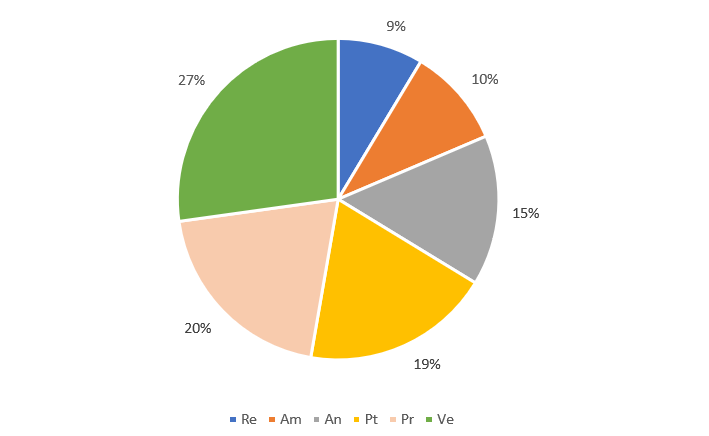
\includegraphics[scale = 0.75]{Immagini/TotaleTorta.png}
    \caption{ Areogramma dei costi totale delle ore di investimento e rendicontate}
    \label{fig:areogramma ripartizione ore totali di investimento e rendicontate}
\end{figure}
\newpage

\subsubsection{Ore rendicontate}
\paragraph{Suddivisione del lavoro}
Nella seguente tabella sono riassunte le ore rendicontate:
\begin{table}[H]
	\begin{center}
		\begin{tabular}{ |c c c c c c c c| }
		\rowcolor{darkblue} 
		\textcolor{white}{\textbf{Nominativo}} & \textcolor{white}{\textbf{Re}} & \textcolor{white}{\textbf{Am}} & \textcolor{white}{\textbf{An}} & \textcolor{white}{\textbf{Pt}} & \textcolor{white}{\textbf{Pr}} & \textcolor{white}{\textbf{Ve}} & \textcolor{white}{\textbf{Ore Complessive}} \\ \hline
		\BL 	& 4  	& 5  	& 8 	& 32 	& 24 	& 27 	& 100 \\ \hline
		\FF 	& 7 	& 5 	& -		& 46 	& 30 	& 12 	& 100 \\ \hline
		\MM 	& 4  	& 11  	& 10 	& 23 	& 26 	& 26  	& 100 \\ \hline
		\PC 	& 10 	& 4  	& 10	& 11 	& 29	& 36 	& 100 \\ \hline
		\TG 	& 5  	& 11 	& 10 	& 19 	& 28 	& 27 	& 100 \\ \hline
		\TL 	& 5  	& 6 	& - 	& 19 	& 32 	& 38 	& 100 \\ \hline
		\VD 	& 18  	& 12  	& -		& 24 	& 24 	& 24 	& 100 \\ \hline
		\textbf{Ore totali} & \textbf{53} & \textbf{54} & \textbf{38} & \textbf{174} & \textbf{191} & \textbf{190} & \textbf{700} \\ \hline
		\end{tabular}
	\caption{Distribuzione delle ore rendicontate}
	\end{center}
\end{table}
I dati ottenuti vengono riassunti nel seguente istogramma:
\begin{figure}[H]
    \centering
    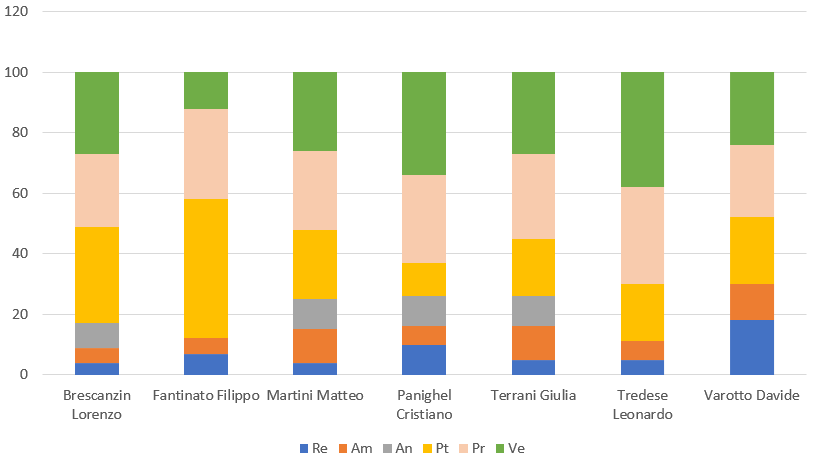
\includegraphics[scale = 0.70]{Immagini/TotaleRendicontatoIsto.png}
    \caption{Istogramma della ripartizione delle ore rendicontate}
    \label{fig:Istogramma ripartizione ore totali rendicontate}
\end{figure}
\newpage
\paragraph{Prospetto economico}
Il costo totale rendicontato per ogni ruolo è il seguente:
\begin{table}[H]
	\begin{center}
		\begin{tabular}{ |c c c| }
		\rowcolor{darkblue} 
		\textcolor{white}{\textbf{Ruolo}} & \textcolor{white}{\textbf{Ore}} & \textcolor{white}{\textbf{Costo}} \\ \hline
		\textit{\Responsabile} 		& 53 	& 1590€ \\ \hline
		\textit{\Amministratore}	& 54 	& 1080€ \\ \hline
		\textit{Analista} 			& 38 	& 950€ \\ \hline
		\textit{Progettista} 		& 174 	& 3828€ \\ \hline
		\textit{Programmatore} 		& 191 	& 2865€ \\ \hline
		\textit{Verificatore} 		& 190 	& 2850€ \\ \hline
		\textbf{Totale} & \textbf{700} & \textbf{13163€} \\ \hline
		\end{tabular}
	\caption{Prospetto delle ore rendicontate}
	\end{center}
\end{table}
Il seguente grafico a torta riassume i dati ottenuti:
\begin{figure}[H]
    \centering
    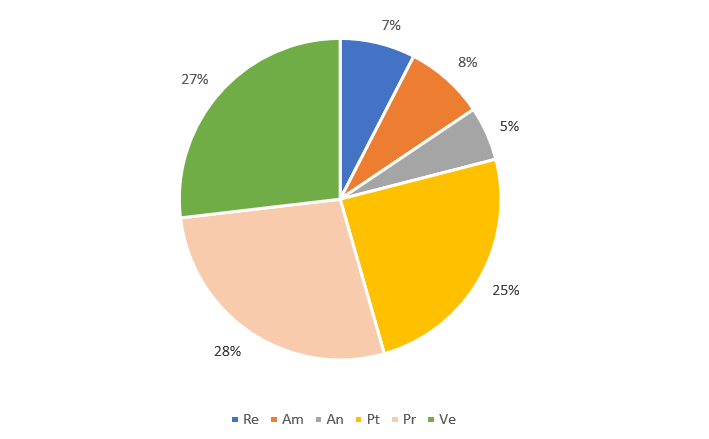
\includegraphics[scale = 0.75]{Immagini/TotaleRendicontatoTorta.png}
    \caption{Areogramma delle ore rendicontate per ruolo}
    \label{fig:Areogramma ripartizione ore totali rendicontate}
\end{figure}
\subsubsection{Conclusioni}
Il costo totale preventivato è: 13163€.